\chapter{Un exemple d'application du profil \emph{Game Genesis}~: Le jeu PUBG}

PUBG est un jeu vidéo, sorti en 2017, qui compte d\'ej\`a des millions d'adeptes à travers le globe. Développé par \emph{PUBG Corporation} (filiale de B\emph{luehole, Inc.}, plus récemment de \emph{Krafton Game Union}), PUBG est un des premiers jeux \emph{standalone}%
\footnote{\ACOMPLETER{D\'ecrire/rappeler bri\`evement ce que signifie <<standalone>>.}}
%
, avec  \emph{Fortnite} (\emph{Epic Games}),
permettant aux joueurs de participer à un <<\emph{Last man standing game}>>. Ces deux jeux ont été les premiers \emph{standalone} à populariser le \emph{Battle Royale} et à le mettre à la portée de tous sans devoir développer ou installer des mods dans des jeux existants.

\GT{Des mods!?}


\section{L'origine des jeux \emph{Battle Royale}}

\GT{Ci-bas: Donner aussi une r\'ef\'erence bibliographiqu pour le roman.}

\GT{Ci-bas: je ne comprends pas <<50 classes de troisi\`eme>>!?}

Les jeux de type \emph{Battle Royale} trouvent leurs racines dans le roman <<\emph{Battle Royale}>>~\cite{ReferencePourLeRomana} et son adaptation cinématographique.%
%
\footnote{\url{https://www.imdb.com/title/tt0266308}}
%
En gros, l'histoire va comme suit.
Un programme militaire de simulation de combat a lieu dans une République socialiste d'Extrême-Orient complètement coupée du monde extérieur, extrêmement stable politiquement, o\`u les habitants n'ont aucun droit civique. Le programme militaire d\'ebute par un tirage au sort annuel de 50 classes de troisième, lesquelles sont déplacées chacune vers une zone de combat. Au début de l'expérience, tous les élèves sont réunis afin de recevoir un briefing rapide, puis se voient attribuer un sac contenant un seul objet (par ex., arme à feu, arme blanche, fourchette, corde de luth, etc). Les \'el\`eves sont ensuite transport\'es et livrés à eux-mêmes dans une zone donnée en ayant pour seule consigne qu'aucune règle n'est imposée\ldots\ et qu'un seul survivant par groupe pourra être gagnant de l'expérience;  les autres devront être exterminés, et ce par n'importe quel moyen. Le champion \AVERIFIER{de chaque groupe} obtient alors le droit de vivre aux frais de l'État pour le reste de ses jours et la reconnaissance comme <<Héros du pays>>.

\section{L'essor de la popularité du \emph{Battle Royale}}
Bien que connu depuis l'ann\'ee 2000, l'intérêt pour le principe du \emph{Battle Royale} n'explose que plus tard, avec le succès de la saga \emph{Hunger Games}%
%
\footnote{\url{https://www.imdb.com/title/tt1392170/}}
%
, mettant en place l'histoire de Katniss Everdeen, une jeune adulte qui participe de son plein gré aux \emph{Hunger Games}. Dans un état totalitaire séparé en castes regroupées dans des districts, deux enfants ou adolescents sont choisis au hasard dans chaque district afin de devenir les Tribus. Ils sont alors réunis dans la capitale et lâchés dans une arène afin de participer à une télé-réalité de match à mort diffusée partout dans le pays.

Le succès des \emph{Hunger Games} a amené les développeurs du jeu \emph{Arma II} à créer un mode de jeu basé sur les mêmes règles. Ce mode sera alors appelé \emph{DayZ} et deviendra par la suite un jeu \emph{standalone}. Un mode voit également le jour : \emph{Battle Royale}. Développé par Brendan Greene tout d'abord pour \emph{Arma II} puis pour \emph{Arma III}, ce mode gagne suffisament en popularité pour qu'il donne naissance au projet de jeu \emph{PlayerUnknown's Battlegrounds} (PUBG) --- \emph{PlayerUnknown} étant le pseudonyme en ligne utilisé par Brendan Greene.

\section{Les règles de PUBG}
Les r\`egles du jeu PUBG vont comme suit.
Un avion parcourt une ligne droite au-dessus d'un territoire, et les 100 joueurs de la partie doivent sauter de cet avion afin d'être parachutés à l'endroit de leur choix --- à condition qu'il soit à portée \AVERIFIER{de parachutage}. Une fois arrivés au sol, les joueurs partent à la recherche d'armes et d'équipements dans des bâtiments et doivent s'exterminer jusqu'à ce qu'un seul joueur soit vivant et gagne ainsi la partie. Il est également possible de jouer en \'equipes de deux ou quatre joueurs, o\`u la dernière équipe encore vivante est l'\'equipe gagnante. Afin de limiter la durée d'une partie, une zone circulaire est définie sur la carte une fois que tous les joueurs ont atterri, et cette zone se réduit au cours de la partie. Les joueurs en dehors de la zone subissent une certaine quantité de dégâts s'ils restent \`a l'ext\'erieur de la zone circulaire, et ces dégâts augmentent au fur et à mesure que le cercle se resserre.

\section{Le \emph{Battle Royale} dans le monde du jeu vidéo}
Ces dernières années, une grande quantité de jeux vid\'eos de type \emph{Battle Royale} ont vu le jour. De \emph{Fortnite} (\emph{Epic Games}) à PUBG, en passant par \emph{Apex Legends} (\emph{Respawn Entertainement}), \emph{Ring of Elysium} (\emph{Tencent Games}) pour ne citer que les plus importants. Des dizaines de jeux voient le jour ou se réinventent afin de coller à la mode du \emph{Battle Royale}. Les plus grandes licences de FPS (\emph{First-Person Shooter}) s'alignent également à cette tendance, et c'est ainsi que voient le jours les modes de jeu \emph{Z1BR} (\emph{H1Z1}), \emph{Firestorm} (\emph{Battlefield V}), \emph{Blackout} (\emph{Call of Duty Black Ops IV}). Mais cette offre répond à une demande phénoménale du public pour ce mode de jeu qui s'impose dans le marché à la même place que les jeux de type MOBA (\emph{Multiplayer Online Battle Arena}), qui étaient des grands favoris du public depuis une dizaine d'années, notamment avec les jeux \emph{League Of Legends} ou \emph{Dota 2}. Avec le temps, les jeux de \emph{Battle Royale} tentent de se réinventer et de trouver de nouveaux publics en gardant le principe du \emph{Battle Royale}, mais en explorant d'autres univers. C'est ainsi que naissent \emph{Last Tide} et son univers aquatique immergé, \emph{Fall Guys : Ultimate Knockout} et son univers coloré où de petits personnages à la physique étrange se battent pour une couronne, \emph{Cuisine Royale}, qui était à l'origine une blague de développeurs mais qui a rencontré un immense succès, dans lequel les personnages se battent à l'aide d'ustensiles de cuisine.

\section{Une description (partielle) des \'el\'ements de \emph{Mechanics} de PUBG}
\subsection{Les données}
Les données concernant les objets de PUBG sont difficile à trouver.
Cependant, certains site internet se sont spécialisés dans l'extraction (\emph{mining}) d'informations à partir des fichiers du jeu.
C'est le cas du \emph{Gamepedia} spécialisé pour PUBG (\url{https://pubg.gamepedia.com/}),
un Wiki régulièrement mis à jour et possédant assez d'informations pour permettre d'identifier les objets du jeu et leurs caractéristiques.
Les données sont toutefois souvent sujettes à modifications au fur et à mesure des mises à jour du jeu.
Cependant, l'exactitude des données n'a pas une importance cruciale dans le cadre du pr\'esent travail.


\subsection{Le profil}

\begin{figure}
    \centering
    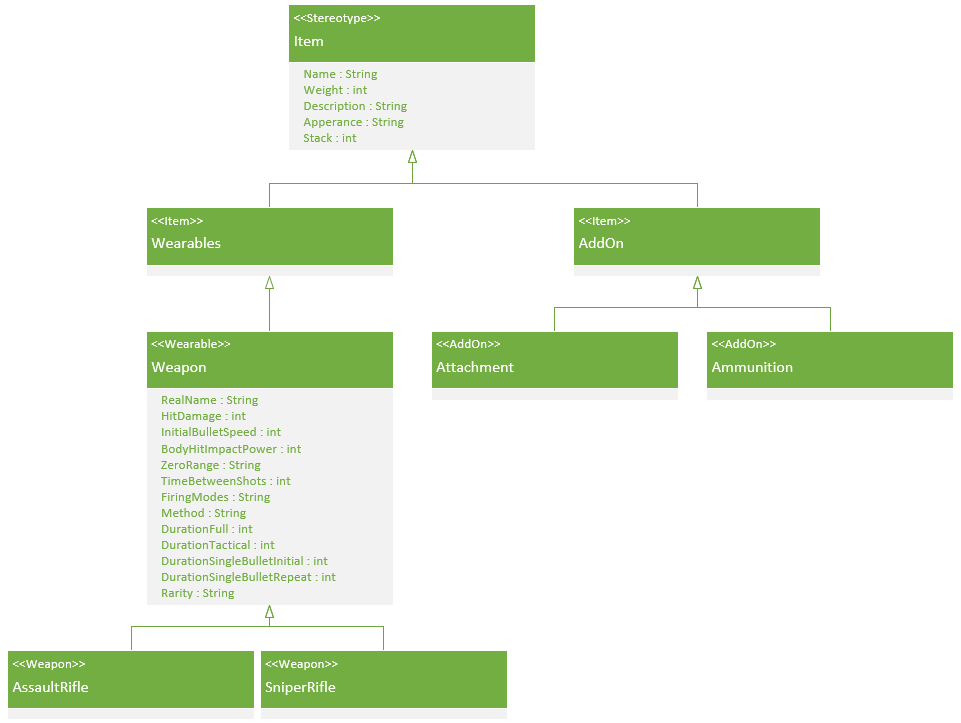
\includegraphics[width=14cm]{10_img/chap6/root(stereotypes).PNG} 
    \caption{Racine des stéréotypes concernés par l'exemple.}
    \label{fig.racine_stereo}
\end{figure}

Les stéréotypes présents dans \emph{Game Genesis} permettent de classifier les \'el\'ements de \emph{Mechanics} pour la rédaction d'un GDD.
Afin de mieux comprendre le fonctionnement de \emph{Game Genesis}, nous avons extrait une partie du profil et la pr\'esentons dans la Figure~\ref{fig.racine_stereo}.
Cette partie du profil inclut les stéréotypes qui sont utilisés dans les exemples présentés dans la suite du chapitre.
De nombreux attributs ont été ajoutés dans les stéréotypes. 
Ceux-ci correspondent aux attributs qui auraient pu être ajoutés par un \emph{game designer} dans le profil.
Ajouter de tels attributs permet d'automatiser la présence des attributs dans les classes créées à partir du profil UML par l'héritage.

\subsection{La modélisation d'un joueur armé}

\begin{figure}
    \centering
    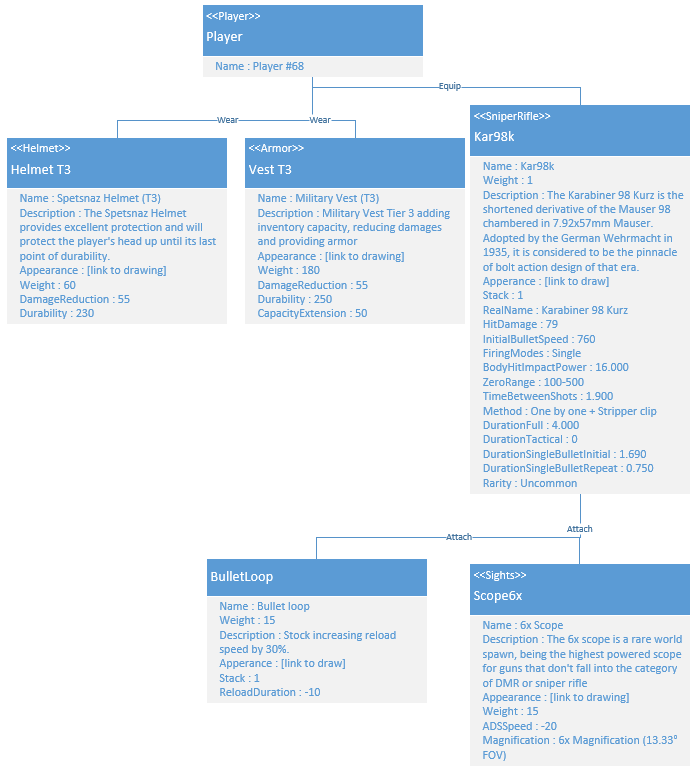
\includegraphics[width=14cm]{10_img/chap6/player68.PNG} 
    \caption{Exemple de modélisation d'un joueur avec son arme.}
    \label{fig.player+weapon+equip}
\end{figure}

La Figure~\ref{fig.player+weapon+equip} présente la modélisation d'un joueur.
Celui-ci est équipé d'un casque \texttt{Tier3} et d'une veste \texttt{T3}. 
Il est armé d'un fusil \emph{sniper} de type \texttt{Kar98k} lui même équipe d'une lunette \texttt{Scope6x} et d'une ceinture de munitions.

Comme décrit \`a la Section~\ref{sect.gg_what}, nous avons utilisé des classes afin de représenter les éléments du jeu, alors que des associations entre classes représentent les interactions entre éléments.
Sur ces classes et associations, nous avons appliqué les stéréotypes du profil UML afin de pouvoir classifier et spécialiser les différents éléments modélisés.



\subsection{La modélisation d'une attaque d'un joueur sur un autre}
\begin{figure}
    \centering
    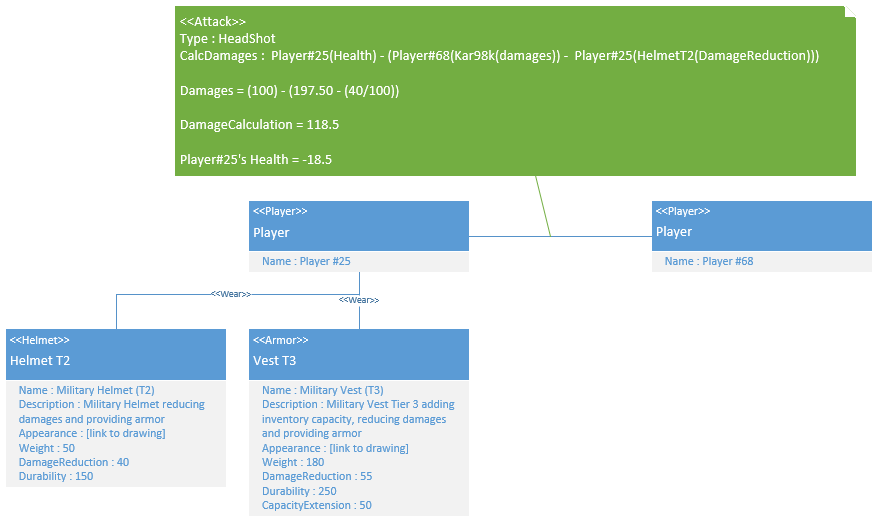
\includegraphics[width=14cm]{10_img/chap6/attack.PNG} 
    \caption{Exemple d'interaction <<~Player68 <<attack>> Player25~>>.}
    \label{fig.attack}
\end{figure}

La Figure~\ref{fig.attack} présente une sp\'ecification d'un joueur qui en attaque un autre.
L'élément \texttt{Player68} est celui modélisé \`a la section précédente.

Le \emph{game designer} a modifié le stéréotype \texttt{attack} afin que celui-ci comprenne le calcul des dégâts d'un joueur sur un autre.
Afin de calculer ces dégâts, nous avons besoin d'un certain nombre d'informations.
Dans un FPS, il est possible d'avoir plusieurs types de dégâts en fonction de l'emplacement de l'attaque.
C'est le cas dans PUBG qui différencie les dégâts en trois types : tête, torse, autres.
Ensuite le calcul des dommages s'effectue en prenant en compte les protections portées par le joueur adverse.
Afin d'exprimer le calcul des dégâts nous avons mis en place la formule suivante :

\begin{equation*}
\begin{split}
Damages& = Attacker(Weapon(Damages(Type(Value)))\\
Protection& = Defender(Protection(DamageReduction))\\
Calcul& = Defender(health) - (Damages - Protection)
\end{split}
%\label{calc.damages}
\end{equation*}

\GT{Ci-haut pour l'\'equation: si par la suite tu ne r\'ef\`eres pas
explicitement \`a cette \'equation, alors pas besoin de lui donner un
num\'ero et un label.}


\GT{Ci-haut et ci-bas: pas besoin de mettre en guillemets si tu
utilises la police appropri\'ee~: \texttt{Attack}.}

Nous retrouvons cette formule de calcul dans la Figure~\ref{fig.attack}.
Elle est présente dans l'association entre les deux joueurs sur laquelle un stéréotype \texttt{Attack} est appliqué.
On considère alors que le \emph{game designer} a modifié le stéréotype de \emph{Game Genesis} afin que toutes les actions d'attaque soient régies par cette formule.

Dans cette figure, il est spécifié que le joueur \texttt{Player68} effectue un tir à la tête sur le joueur \texttt{Player25}.
Le calcul des dommages renvoie un résultat de 118.5 points de dégats.
Le joueur \texttt{Player25} ne possède cependant que 100 points de vie (\texttt{Health}).
On peut donc considérer qu'à la suite de cette action d'attaque, le joueur \texttt{Player25} est éliminé, 
ce qui peut être exprimé par les contraintes suivantes~: 

{
\footnotesize
\begin{framed}
    Player(health) : is max 100.\\
    (IF Player(health) < 0)\\
    \{\\
    IF Gamemode is "solo" ==> Player is dead and eliminated.\\
    IF Gamemode is "duo" OR "squad" ==> Player is knocked.\\
    \}
\end{framed}
}

\section{Conclusion}
